\chapter{Fundamentação Teórica}

\section{Métodos Utilizados}
\subsection{Método de Newton}

Pode ser necessário utilizar uma figura para explicar alguma coisa, tal como mostrar algum método, como o método de Newton para aproximação de uma função, que consiste em realizar esta aproximação através da função tangente, como mostra a figura

\begin{figure}[H]
    \centering
    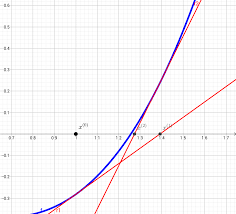
\includegraphics{Imagens/newton-method.png}
    \caption{Exemplo de utilização do método de Newton}
    \label{fig:newton}
\end{figure}

A tag [H] serve para posicionar a figura na posição exata do texto, caso contrário, a mesma poderá aparecer como objeto flutuante em regiões indesejadas devido a erros no LaTEX.
Para referenciar a figura, basta utilizar o comando ref, desta forma: \ref{fig:newton}


